\documentclass[a4paper,12pt]{article}
\usepackage[margin=1in]{geometry}
\usepackage{enumitem}
\usepackage{parskip}
\usepackage{titlesec}
\usepackage{graphicx}
\usepackage{amssymb}
\usepackage{tikz}
\usetikzlibrary{shapes.geometric, arrows.meta, positioning}

% Adjust section formatting to look more like form headers
\titleformat{\section}
  {\normalfont\large\bfseries}{\thesection}{1em}{}
\titlespacing*{\section}{0pt}{1.5ex plus 1ex minus .2ex}{0.5ex plus .2ex}

\begin{document}

% --- Header ---
\begin{center}
    \textbf{\Large RV College of Engineering} \\
    Bangalore \\
    \textbf{IP Cell} \\
    \vspace{0.5cm}
    \textbf{\Large Invention Disclosure Form (IDF)}
\end{center}

\vspace{0.5cm}

% --- Reference Information ---
\noindent \textbf{Invention No:} RVCE-CSE-MP-001 \hfill \textbf{Version:} 01

\hrulefill

% ============================================================================
% SECTION 1: TITLE
% ============================================================================
\section*{Title of the Invention}

\textbf{An Interpretable Clinical Framework for Ingredient-Level Dietary Portion Recommendation in Hypertension, Diabetes Mellitus, and Chronic Kidney Disease Using Clinical Risk Stratification and Nutrient Constraint Logic}

% ============================================================================
% SECTION 2: INVENTORS
% ============================================================================
\section*{Name, Designation, Department, Email ID and Phone No. of the Inventors}

\begin{enumerate}
    \item \textbf{Mri Pradhan} \\
    Student, Department of Computer Science and Engineering \\
    Email: \texttt{mripradhan.cs23@rvce.edu.in} \\
    Phone: \textit{[To be filled]}
\end{enumerate}

\textit{(Add additional inventors as applicable.)}

% ============================================================================
% SECTION 3: RESIDENTIAL ADDRESS
% ============================================================================
\section*{Residential Address of All the Inventors}

\begin{enumerate}
    \item Mri Pradhan \\
    \textit{[To be filled with residential address]}
\end{enumerate}

% ============================================================================
% SECTION 4: BRIEF DESCRIPTION
% ============================================================================
\section*{Brief Description --- What Does It Do? How Does It Do It?}

The invention is an \textbf{interpretable clinical framework} that computes \textbf{ingredient-level dietary portion recommendations} for patients simultaneously diagnosed with \textbf{Hypertension (HTN)}, \textbf{Type~2 Diabetes Mellitus (T2DM)}, and \textbf{Chronic Kidney Disease (CKD)}. The framework uses a \textbf{clinical risk stratification} hierarchy to resolve conflicting nutrition guidelines across co-existing conditions and applies \textbf{nutrient constraint logic} to determine safe, per-ingredient portion sizes --- with every recommendation accompanied by an \textbf{interpretable clinical rationale} citing specific patient lab values and evidence-based guidelines.

\medskip
\noindent\textbf{What it does:}
\begin{itemize}[itemsep=0.3em]
    \item For each ingredient available to a patient, the system computes a \textbf{clinically safe portion (in grams)} by evaluating the ingredient's nutrient profile against the patient's personalized daily and per-meal limits for potassium, sodium, phosphorus, protein, and carbohydrates.
    \item Uses a \textbf{clinical risk stratification} hierarchy (Renal $>$ Cardiac $>$ Metabolic $>$ Lipid $>$ Endocrine $>$ General) to automatically \textbf{resolve conflicting dietary guidelines}. For example, when HTN recommends high potassium (DASH diet) but CKD demands potassium restriction, the framework applies a hard cap based on renal severity and documents the override rationale.
    \item Every portion recommendation is \textbf{fully interpretable}: the system generates explainability logs that cite the patient's specific lab values (e.g., ``eGFR~52~mL/min/1.73m$^2$ $\Rightarrow$ K$^+$~$\leq$~650~mg/meal''), the clinical guideline applied (KDOQI, ADA, AHA/ACC), and the priority level of the ruling constraint.
    \item Processes available ingredients via computer vision scan input, maps each to the USDA FoodData Central nutrient database, and classifies them as \textbf{safe}, \textbf{restricted} (capped portion), or \textbf{prohibited} (with safer alternatives suggested).
    \item Downstream, the portion recommendations drive recipe adaptation using a structured \textbf{SHARE methodology} (Substitute, Halve, Add, Remove, Emphasize) for clinically compliant meal generation.
\end{itemize}

\medskip
\noindent\textbf{How it does it:}

The framework operates as a \textbf{five-stage automated pipeline}:
\begin{enumerate}[itemsep=0.3em]
    \item \textbf{Patient Clinical Profiling} --- Extracts demographics, diagnoses (ICD-coded), and 14 lab parameters from MIMIC-IV electronic health records.
    \item \textbf{Clinical Risk Stratification \& Nutrient Constraint Generation} --- The hierarchical rules engine stratifies clinical risk, resolves inter-condition conflicts, and outputs personalized nutrient limits (daily and per-meal) as a structured ClinicalConstraint.
    \item \textbf{Ingredient-Level Portion Computation} --- Each pantry ingredient is mapped to USDA FDC nutrients and its safe portion is computed against the ClinicalConstraint, yielding per-ingredient gram-level recommendations.
    \item \textbf{Interpretable Recipe Adaptation} --- Portion-constrained ingredients are assembled into clinically adapted meals via the SHARE methodology, with full explainability logs.
    \item \textbf{Safety Validation \& Reporting} --- Multi-layer compliance checks and a final interpretable report with safety alerts.
\end{enumerate}

% ============================================================================
% SECTION 5: DETAILS OF THE INVENTION
% ============================================================================
\section*{Details of the Invention}

\subsection*{Module 1: MIMIC-IV Patient Extraction (\texttt{mimic\_cohort\_extraction.py})}
\begin{itemize}[itemsep=0.3em]
    \item Extracts cohort of patients with the three target conditions (HTN, T2DM, CKD) --- and optionally Dyslipidemia --- using ICD-9/ICD-10 codes.
    \item Retrieves \textbf{14 laboratory parameters} essential for risk stratification: eGFR, serum potassium (K$^+$), HbA1c, serum creatinine, BUN, serum phosphorus, total cholesterol, LDL, HDL, triglycerides, fasting glucose, serum albumin, hemoglobin, and TSH.
    \item Performs weight-based calculations (for protein requirement computation) with fallback to reference weight (70\,kg) when unavailable.
    \item Computes data completeness metrics for each patient profile to ensure downstream constraint logic has reliable inputs.
    \item \textbf{Novelty}: Structured extraction of lab parameters specifically selected to feed the clinical risk stratification hierarchy and nutrient constraint logic, with completeness tracking to flag unreliable inputs.
\end{itemize}

\subsection*{Module 2: Clinical Risk Stratification \& Nutrient Constraint Engine (\texttt{clinical\_rules\_engine.py})}

This is the \textbf{core novel component} of the invention --- the \textbf{clinical risk stratification} and \textbf{nutrient constraint logic} referenced in the title.

\begin{itemize}[itemsep=0.3em]
    \item Implements a \textbf{six-level clinical priority hierarchy}:
    \begin{enumerate}
        \item \textbf{CRITICAL\_RENAL} (Priority 1) --- Life-threatening electrolyte imbalances
        \item \textbf{CRITICAL\_CARDIAC} (Priority 2) --- Cardiovascular risk factors
        \item \textbf{HIGH\_METABOLIC} (Priority 3) --- Glycemic control
        \item \textbf{MEDIUM\_LIPID} (Priority 4) --- Lipid management
        \item \textbf{LOW\_ENDOCRINE} (Priority 5) --- Thyroid and hormonal
        \item \textbf{GENERAL\_HEALTH} (Priority 6) --- Baseline nutrition
    \end{enumerate}

    \item \textbf{Critical Conflict Resolution --- Potassium Example:}
    \begin{itemize}
        \item HTN guideline (DASH diet) recommends \textbf{high potassium} ($\geq 4700$\,mg/day).
        \item CKD guideline requires \textbf{low potassium} ($\leq 2000$\,mg/day) to prevent life-threatening hyperkalemia.
        \item \textbf{Resolution}: When eGFR $< 60$\,mL/min/1.73m$^2$ (CKD Stage 3--5), the engine applies a \textbf{hard cap} of 2000\,mg/day, overriding the HTN guideline. The override is documented with clinical rationale.
    \end{itemize}

    \item Generates a structured \textbf{ClinicalConstraint JSON} output containing:
    \begin{itemize}
        \item Daily and per-meal nutrient limits (sodium, potassium, phosphorus, protein)
        \item Prohibited foods list with alternatives
        \item Limited foods with capped quantities
        \item Temporal warnings (e.g., soy--levothyroxine 4-hour spacing)
        \item Conflict resolution audit trail
    \end{itemize}

    \item \textbf{Key sub-functions}:
    \begin{itemize}
        \item \texttt{classify\_ckd\_stage()}: CKD staging based on eGFR thresholds (KDIGO 2017)
        \item \texttt{resolve\_potassium\_conflict()}: Renal vs. HTN conflict resolution
        \item \texttt{resolve\_food\_restrictions()}: Food-level clinical restrictions
        \item \texttt{calculate\_protein\_requirements()}: Weight-based protein targets (KDOQI 2020)
        \item \texttt{calculate\_sodium\_limit()}: Condition-specific sodium management
        \item \texttt{calculate\_phosphorus\_limit()}: CKD-stage phosphorus control
    \end{itemize}

    \item \textbf{Novelty}: No existing system provides automated, priority-based \textbf{clinical risk stratification} that resolves inter-condition nutrient conflicts and outputs \textbf{interpretable, ingredient-level portion constraints} with a documented audit trail. Existing dietary tools either handle single conditions or require manual clinician input for conflict resolution. The interpretability --- every constraint traces to a specific lab value, guideline, and priority level --- is a key differentiator.
\end{itemize}

\subsection*{Module 3: Ingredient-Level Portion Recommendation Engine (\texttt{pantry\_inventory.py})}
\begin{itemize}[itemsep=0.3em]
    \item Processes simulated \textbf{Computer Vision (CV) scans} of a patient's pantry to identify available ingredients.
    \item \textbf{Normalizes CV labels} to standardized food names (handles synonyms, abbreviations).
    \item Maps each ingredient to the \textbf{USDA FoodData Central (FDC)} nutrient database via API, retrieving per-100g nutrient profiles (potassium, sodium, protein, carbohydrates, phosphorus, calories, fiber, saturated fat).
    \item \textbf{Computes ingredient-level safe portions}: For each ingredient, the module calculates the maximum allowable quantity (in grams) by evaluating its nutrient density against the patient's per-meal and daily nutrient ceilings from the ClinicalConstraint. For example, if a patient's per-meal potassium limit is 650\,mg and carrots contain 320\,mg K$^+$/100g, the safe portion is capped at $\approx$200\,g.
    \item Classifies each ingredient with an \textbf{interpretable status}:
    \begin{itemize}
        \item \textbf{Safe}: Ingredient is allowed; computed portion is within clinical limits.
        \item \textbf{Restricted}: Ingredient exceeds limits at scanned quantity; \textbf{portion is capped} with an interpretable warning citing the binding nutrient constraint.
        \item \textbf{Prohibited}: Ingredient is clinically dangerous at any quantity; flagged with safer alternatives from the rules engine.
    \end{itemize}
    \item Generates a \textbf{PantrySummary} JSON with per-ingredient portion recommendations, nutrient breakdowns, warnings, and clinical rationale.
    \item \textbf{Novelty}: The system performs \textbf{ingredient-level dietary portion computation} --- not just food classification --- by cross-referencing USDA nutrient densities against patient-specific nutrient ceilings derived from clinical risk stratification. Each portion recommendation is accompanied by an interpretable rationale.
\end{itemize}

\subsection*{Module 4: Interpretable Recipe Adaptation via SHARE Methodology (\texttt{recipe\_generator.py})}

This module consumes the ingredient-level portion recommendations to assemble clinically compliant meals.

\begin{itemize}[itemsep=0.3em]
    \item Uses \textbf{Retrieval-Augmented Generation (RAG)} to search for recipes matching the patient's available (and portion-constrained) pantry ingredients.
    \item Applies the \textbf{SHARE methodology} for clinical recipe adaptation, operating on the portion recommendations from Module~3:
    \begin{itemize}
        \item \textbf{S}ubstitute --- Replace prohibited ingredients with clinically safe alternatives (e.g., potato $\rightarrow$ cauliflower for CKD patients)
        \item \textbf{H}alve --- Enforce the computed portion caps on restricted ingredients (e.g., reduce salt portion for HTN)
        \item \textbf{A}dd --- Introduce beneficial nutrients to meet minimum thresholds (e.g., add chia seeds for fiber/diabetes)
        \item \textbf{R}emove --- Eliminate prohibited items entirely
        \item \textbf{E}mphasize --- Highlight critical clinical information (e.g., carb counting for diabetics, low-oil cooking methods for dyslipidemia)
    \end{itemize}
    \item Generates \textbf{interpretable explainability logs} that trace each recipe modification to:
    \begin{itemize}
        \item The specific patient lab value that triggered the constraint (e.g., ``eGFR 52 mL/min/1.73m$^2$ $\Rightarrow$ K$^+$ restriction'')
        \item The clinical guideline applied (KDOQI 2020, ADA 2024, AHA/ACC 2017)
        \item The clinical risk stratification priority level that governed the decision
    \end{itemize}
    \item Validates final adapted recipes against clinical constraints (post-adaptation compliance check with violation reporting).
    \item \textbf{Novelty}: The SHARE methodology is a structured, repeatable framework for translating ingredient-level portion constraints into complete, adapted meals. Combined with lab-value-citing interpretability, it provides a level of clinical transparency absent in existing dietary software.
\end{itemize}

\subsection*{Module 5: Interpretable Safety Reporting \& System Integration (\texttt{main\_integration.py})}
\begin{itemize}[itemsep=0.3em]
    \item Orchestrates all four modules as a single automated pipeline.
    \item Generates a comprehensive \textbf{Interpretable Final Report} including: clinical risk stratification summary, per-ingredient portion recommendations with rationale, safety alerts (CRITICAL/HIGH/MEDIUM/LOW), adapted recipe summaries, and recommended next steps.
    \item Multi-layer validation at every stage: pre-generation clinical risk checks, per-ingredient portion constraint verification, and post-adaptation compliance validation.
    \item Every output is \textbf{fully traceable}: a clinician or patient can follow the chain from a specific lab value $\rightarrow$ risk stratification level $\rightarrow$ nutrient constraint $\rightarrow$ ingredient portion cap $\rightarrow$ recipe modification.
\end{itemize}

\subsection*{How Modules Interact}

\begin{center}
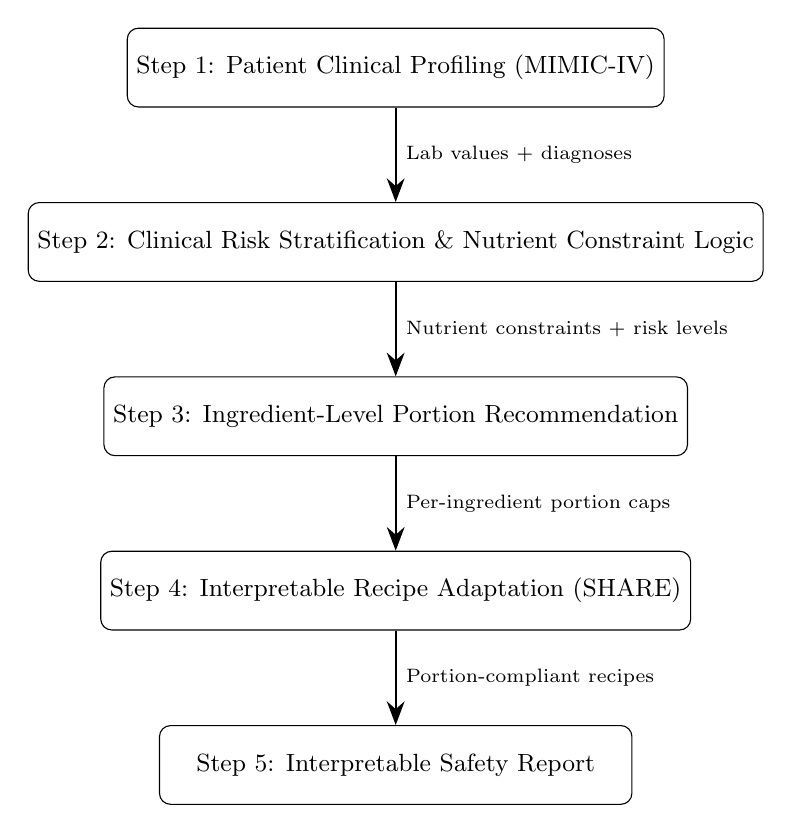
\begin{tikzpicture}[
    node distance=1.2cm,
    block/.style={rectangle, draw, rounded corners, text centered, minimum width=6cm, minimum height=1cm, font=\small},
    arrow/.style={-{Stealth[length=3mm]}, thick}
]
    \node[block] (step1) {Step 1: Patient Clinical Profiling (MIMIC-IV)};
    \node[block, below=of step1] (step2) {Step 2: Clinical Risk Stratification \& Nutrient Constraint Logic};
    \node[block, below=of step2] (step3) {Step 3: Ingredient-Level Portion Recommendation};
    \node[block, below=of step3] (step4) {Step 4: Interpretable Recipe Adaptation (SHARE)};
    \node[block, below=of step4] (step5) {Step 5: Interpretable Safety Report};

    \draw[arrow] (step1) -- node[right, font=\scriptsize] {Lab values + diagnoses} (step2);
    \draw[arrow] (step2) -- node[right, font=\scriptsize] {Nutrient constraints + risk levels} (step3);
    \draw[arrow] (step3) -- node[right, font=\scriptsize] {Per-ingredient portion caps} (step4);
    \draw[arrow] (step4) -- node[right, font=\scriptsize] {Portion-compliant recipes} (step5);
\end{tikzpicture}
\end{center}

% ============================================================================
% SECTION 6: PROBLEM SOLVED AND ADVANTAGES
% ============================================================================
\section*{Please Briefly Describe the Problem That the Technology Solves and Its Advantages/Benefits Relative to Competing Technologies or Products}

\subsection*{Problem}
Patients with \textbf{co-existing Hypertension, Diabetes Mellitus, and Chronic Kidney Disease} face \textbf{conflicting dietary guidelines} that make ingredient-level dietary decisions extremely difficult:
\begin{itemize}[itemsep=0.3em]
    \item \textbf{Potassium conflict}: HTN treatment recommends high potassium ($\geq$4700~mg/day via DASH diet), while CKD management requires potassium restriction ($\leq$2000~mg/day) to avoid fatal hyperkalemia. A dietitian must determine \textit{exactly how many grams} of a potassium-containing ingredient is safe.
    \item \textbf{Protein conflict}: Diabetes benefits from adequate protein for glycemic control, while CKD requires protein restriction (0.6--0.8~g/kg/day) to slow renal decline. The safe portion of a protein-rich ingredient depends on multiple lab values simultaneously.
    \item \textbf{No automated portion computation}: Current clinical nutrition tools provide general food-category guidance (``limit potassium'') but do not compute \textbf{specific gram-level portions} for individual ingredients based on the patient's actual lab values.
    \item \textbf{No interpretability}: When dietary tools do make recommendations, they provide no traceable rationale connecting the recommendation to specific lab values and clinical guidelines, making it difficult for clinicians to verify safety.
\end{itemize}

\subsection*{Advantages Over Existing Technologies}
\begin{enumerate}[itemsep=0.3em]
    \item \textbf{Ingredient-Level Portion Recommendation}: Unlike existing tools that provide food-category guidance, this framework computes \textbf{exact safe portions in grams} for each ingredient based on the patient's nutrient constraints.
    \item \textbf{Clinical Risk Stratification}: A six-level priority hierarchy automatically resolves inter-condition conflicts without manual dietitian intervention, reducing workload and eliminating human error.
    \item \textbf{Full Interpretability}: Every portion recommendation and dietary decision is traceable from lab value $\rightarrow$ risk level $\rightarrow$ nutrient constraint $\rightarrow$ portion cap, enabling physician verification and patient education.
    \item \textbf{Nutrient Constraint Logic}: Formal, evidence-based constraint rules (not heuristics or black-box ML) ensure deterministic, reproducible, and auditable recommendations.
    \item \textbf{Real Clinical Data}: Uses actual MIMIC-IV patient records with 14 lab parameters, ensuring clinical accuracy.
    \item \textbf{Pantry-Aware Computation}: Leverages computer vision and USDA nutrient densities to compute portions from ingredients the patient \textit{actually has}, improving compliance.
    \item \textbf{Multi-Layer Safety}: Three validation layers (pre-generation risk checks, per-ingredient portion verification, post-adaptation compliance) ensure no unsafe dietary recommendation is generated.
\end{enumerate}

% ============================================================================
% SECTION 7: POTENTIAL PRODUCT
% ============================================================================
\section*{What Product Might This Invention Become?}

\begin{enumerate}[itemsep=0.3em]
    \item \textbf{Clinical Decision Support Tool}: Integrated into Electronic Health Record (EHR) systems to assist dietitians and nephrologists with automated meal planning for multi-morbid patients.
    \item \textbf{Patient-Facing Mobile Application}: A smartphone app where patients scan their pantry with a camera, input their lab values, and receive safe, personalized meal plans with full clinical explanations.
    \item \textbf{Hospital Nutrition Management System}: Deployed in hospital food service departments to automatically generate compliant meals for inpatients with complex dietary needs.
    \item \textbf{Telehealth Nutrition Platform}: A SaaS product for remote dietitian consultations, providing automated constraint analysis and recipe suggestions as a baseline for clinical review.
    \item \textbf{Smart Kitchen Integration}: Connected to smart refrigerators/pantry systems that automatically track inventory and suggest safe recipes based on the patient's current clinical status.
\end{enumerate}

% ============================================================================
% SECTION 8: ALTERNATIVES AND LIMITATIONS
% ============================================================================
\section*{Alternatives and Limitations of the Proposed Invention}

\subsection*{Alternative Approaches}
\begin{itemize}[itemsep=0.3em]
    \item \textbf{Machine Learning Approach}: A purely ML-based model could learn optimal meal plans from historical dietitian recommendations. However, this approach lacks explainability (black-box predictions) and requires extensive labeled training data that does not currently exist for multi-morbid patients.
    \item \textbf{Ontology-Based Reasoning}: Using formal medical ontologies (SNOMED-CT, RxNorm) for dietary rule encoding. This would provide semantic richness but at the cost of significant complexity and slower execution.
    \item \textbf{LLM-Only Generation}: Using large language models (e.g., GPT-4, Claude) to directly generate meal plans. This lacks the deterministic safety guarantees of rule-based conflict resolution and can hallucinate unsafe recommendations.
\end{itemize}

\subsection*{Limitations}
\begin{itemize}[itemsep=0.3em]
    \item Currently validated for four specific conditions (HTN, T2DM, CKD, Dyslipidemia); additional conditions (e.g., Heart Failure, Celiac Disease) require new rule definitions.
    \item CV-based pantry scanning is currently simulated; real-world deployment requires integration with actual computer vision models.
    \item USDA FDC nutrient data is US-centric; Indian food databases (IFCT 2017) are being integrated but are not yet fully operational.
    \item Recipe database is currently a curated sample; production deployment requires integration with large-scale recipe APIs.
    \item The system does not account for patient taste preferences, cultural dietary restrictions, or food allergies (these can be added as additional constraint layers).
\end{itemize}

% ============================================================================
% SECTION 9: CURRENT STATE OF ART
% ============================================================================
\section*{Current State of Art}

\subsection*{How Is This Problem Being Solved Today?}
Currently, ingredient-level dietary portion decisions for patients with HTN, DM, and CKD rely on \textbf{manual dietitian consultation}. A registered dietitian reviews the patient's lab values, mentally resolves conflicts between condition-specific guidelines, and estimates safe portions. This process is:
\begin{itemize}
    \item Time-intensive (30--60 minutes per patient)
    \item Error-prone when resolving 3+ conflicting guideline sets simultaneously
    \item Inconsistent between practitioners (no standardized conflict resolution protocol)
    \item Not scalable to large patient populations
    \item Lacking in interpretable documentation of the reasoning chain
\end{itemize}

\subsection*{Nearest Existing Systems}
\begin{itemize}[itemsep=0.3em]
    \item \textbf{Nutritics / Computrition}: Hospital nutrition software that provides nutrient analysis but \textit{does not} compute ingredient-level portions or resolve conflicts between conditions. Requires manual dietitian input.
    \item \textbf{MyFitnessPal / Cronometer}: Consumer calorie-tracking apps with no clinical risk stratification. Cannot handle CKD-specific potassium limits or inter-condition conflicts.
    \item \textbf{Prospre / Eat This Much}: AI meal planning tools that optimize for single wellness goals (weight loss, muscle gain) but have no clinical constraint logic or multi-condition support.
    \item \textbf{Research systems}: Some academic systems address single-condition dietary planning, but none implement a formalized clinical risk stratification hierarchy for multi-condition nutrient constraint resolution with interpretable output.
\end{itemize}

\subsection*{How Does This Invention Differ?}
\begin{enumerate}[itemsep=0.3em]
    \item \textbf{No existing system} computes \textbf{ingredient-level dietary portions} (gram-level) using formalized nutrient constraint logic derived from patient-specific lab values.
    \item \textbf{No existing system} implements \textbf{clinical risk stratification} with priority-based conflict resolution across HTN, DM, and CKD simultaneously.
    \item \textbf{No existing system} provides \textbf{interpretable} portion recommendations where every decision is traceable from lab value to guideline to risk level to portion cap.
    \item \textbf{No existing system} integrates real EHR data (MIMIC-IV) directly into an ingredient-level portion recommendation pipeline.
    \item \textbf{No existing system} combines USDA nutrient density data with clinical nutrient ceilings to compute per-ingredient safe quantities in an automated framework.
\end{enumerate}

\subsection*{References}
\begin{enumerate}[itemsep=0.3em]
    \item Johnson, A., Bulgarelli, L., Pollard, T., et al. (2023). \textit{MIMIC-IV (version 2.2)}. PhysioNet. \texttt{https://doi.org/10.13026/6mm1-ek67}
    \item KDOQI Clinical Practice Guideline for Nutrition in CKD: 2020 Update. \textit{Am J Kidney Dis.} 76(3):S1--S107.
    \item American Heart Association / American College of Cardiology Hypertension Guidelines (2017).
    \item American Diabetes Association. Standards of Medical Care in Diabetes---2024. \textit{Diabetes Care.} 47(Suppl 1).
    \item KDIGO 2012 Clinical Practice Guideline for the Evaluation and Management of Chronic Kidney Disease. \textit{Kidney International Supplements.} 3(1).
    \item U.S. Department of Agriculture, FoodData Central. \texttt{https://fdc.nal.usda.gov/}
    \item \textit{Indian Food Composition Tables (IFCT 2017)}, National Institute of Nutrition, ICMR.
\end{enumerate}

% ============================================================================
% SECTION 10: PUBLIC DISCLOSURES
% ============================================================================
\section*{Public Disclosures}

\begin{enumerate}[itemsep=0.3em]
    \item Is this invention or work published in any journal, conference, seminar, workshop or any public meeting? \\
    \textbf{No.} The work has not been published in any journal, conference, or public forum.

    \item Is this work or invention sent to any competition? \\
    \textbf{Yes.} This project was submitted as a semifinalist entry to the \textbf{Unisys Innovation Program Year 16 (Y16)}. No detailed technical disclosure of the algorithm or methodology was made publicly.

    \item Is this work presented to customers? \\
    \textbf{No.}

    \item Is this work submitted to any funding agencies? \\
    \textbf{No.}
\end{enumerate}

% ============================================================================
% SECTION 11: COMMERCIAL POTENTIAL
% ============================================================================
\section*{Commercial Potential}

\textbf{Mention possible products, solutions, services that can be made from this invention:}
\begin{itemize}[itemsep=0.3em]
    \item \textbf{Clinical Decision Support SaaS}: Subscription-based software for hospitals and nephrology clinics.
    \item \textbf{Patient Mobile App}: Direct-to-consumer app for CKD/Diabetes patients with pantry scanning.
    \item \textbf{API Service}: Nutrition constraint engine as a microservice for integration into existing EHR platforms (Epic, Cerner, etc.).
    \item \textbf{Hospital Food Service Automation}: Tray-management systems for inpatient meal production.
    \item \textbf{Insurance Wellness Programs}: Disease-management nutrition tool for health insurers to reduce hospitalization costs.
\end{itemize}

\vspace{0.5cm}

\textbf{Mention the companies or industries that are most likely to be interested in this technology:}
\begin{itemize}[itemsep=0.3em]
    \item \textbf{Healthcare IT}: Epic Systems, Cerner (Oracle Health), Medidata, Practo (India)
    \item \textbf{Hospital Nutrition}: Sodexo Healthcare, Aramark, Compass Group
    \item \textbf{Health Tech Startups}: Noom, Virta Health, Livongo (Teladoc)
    \item \textbf{Consumer Health}: Apple Health, Google Health, Samsung Health
    \item \textbf{Pharma/Diagnostics}: Abbott (FreeStyle Libre), DaVita (Renal Care)
    \item \textbf{Insurance}: UnitedHealth, Star Health (India), ICICI Lombard
\end{itemize}

\vspace{0.5cm}

\textbf{Mention which of the following best describes your invention disclosure:}
\begin{itemize}[noitemsep]
    \item [$\boxtimes$] Has significant commercial value
    \item [$\boxtimes$] Is a method or platform or technology that can go to existing product, solution or services
    \item [$\boxtimes$] Particular company may be interested in this invention
    \item [$\square$] I/we can start a start-up company using this invention
\end{itemize}

\end{document}
